\subsubsection{Wersja YAML}
Finalną wersję pipeline'a umieściłem bezpośrednio w repozytorium jako pliki YAML w folderze \verb|CI|.
Korzystając z możliwości Azure podzieliłem duży plik zawierający wszystkie kroki 
na pomniejsze template'y (szablony), które mogę ponownie wykorzystać w dowolnie dużej 
ilości i kolejności.

Cała struktura zadań podzielona jest na kilka grup - tworząc je możemy zacząć od etapów (ang. stage), 
wewnątrz nich zawrzeć kilka jobów (prac, zadań), które składają się z kroków wykonania (ang. steps).


\begin{figure}[ht]
    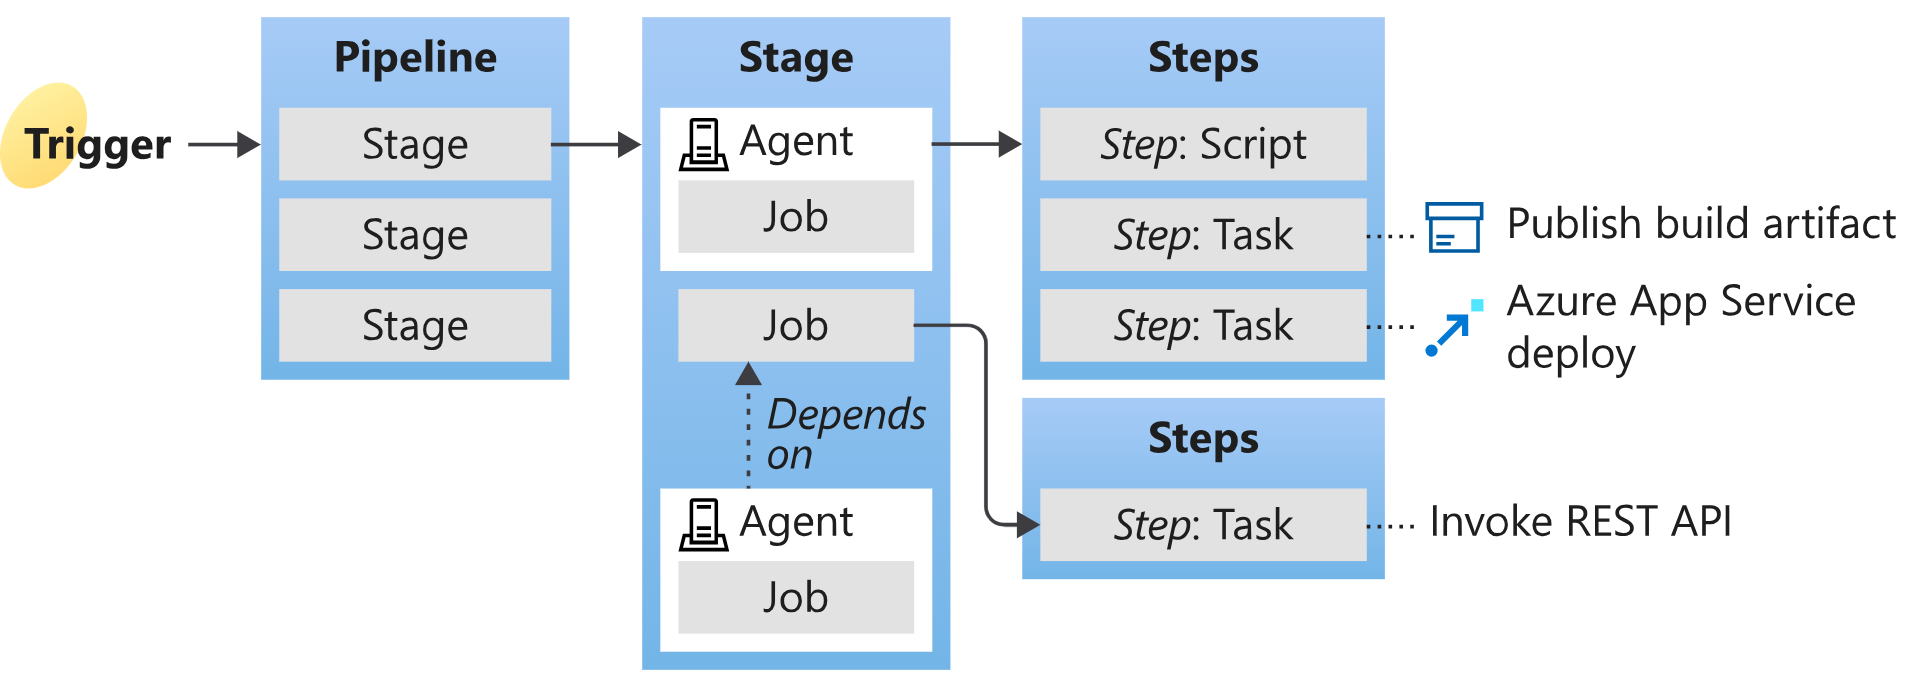
\includegraphics[width=\textwidth]{pipelineSchemaAzure.png}
    \caption{Hierarchia etapów i zadań w Azure~\cite{pipelineSchemaAzure_source}}
    \label{img:pipelineSchemaAzure}
    
\end{figure}
